\documentclass[twocolumn]{article}
\usepackage{graphicx}
\usepackage{amsmath}
\usepackage{float}
\usepackage{amssymb} %Use of therefore symbol
\usepackage{hyperref}
\usepackage{caption}



\begin{document}
\title{Assignment 2: Fourier Analysis}
\author{Alex Matheson, Austin Nhung}
%\affiliation{Department of Physics and Astronomy, University of Calgary, Calgary AB T2N 1N4 Canada}
\date{\today}
\maketitle

\section{Introduction}
The Fourier transform is the cornerstone of modern computing, allowing underlying patterns to be found in big data. For a practical use of Fourier analysis, the discrete Fourier transform (DFT) is used in the modern digital world. Advances in algorithms classed as fast Fourier transforms (FFT) have made the use of Fourier analysis on digital platforms practical. This assignment will explore the aforementioned aspects of Fourier analysis: the DFT, the FFT, and real-world applications. Applications can include any sort of data analysis where periodicity is expected. This will include astrophysical systems, physiological systems, financial systems, and the Earth's climate.

\subsection{DFT vs FFT}
The discrete fourier transform allows a discrete set of data to be transformed according to the equation:
\begin{equation}
X(f) = \sum_{n=0}^{N-1} x_n e^{2\pi ink/N}
\end{equation}

When data are sampled in the real world, a generally continuous function is divided into discrete samples. Consider the continuous function:
\begin{equation}
X(\omega) = \begin{cases}
1, \quad |\omega| \leq \frac{\pi}{3} \\
0, \quad otherwise
\end{cases}
\end{equation}

This function may be sampled at given frequency intervals $\Delta \omega = 1$ to give a series of four data points. From this, the inverse discrete transform may be taken to determine the discrete time spectrum. 
\begin{equation}
\begin{split}
x(t) &= \frac{1}{N} W^{\omega t}_N X(\omega) \\
&= \frac{1}{N} \begin{bmatrix}
W^{00} & W^{01} & W^{02} & W^{03} \\
W^{10} & W^{11} & W^{12} & W^{13} \\
W^{20} & W^{21} & W^{22} & W^{23} \\
W^{30} & W^{31} & W^{32} & W^{33} \\
\end{bmatrix} \begin{bmatrix}X(0) \\ X(1) \\ X(2) \\ X(3)\end{bmatrix} \\
&= \frac{1}{4} \begin{bmatrix}
1 & 1 & 1 & 1 \\
1 & i & -1 & -i \\
1 & -1 & 1 & -1 \\
1 & -i & -1 & i \\
\end{bmatrix} \begin{bmatrix}1 \\ 1 \\ 0 \\ 0\end{bmatrix} \\
&= \frac{1}{4} \begin{bmatrix}2 \\ 1+i \\ 0 \\ 1-i\end{bmatrix} \\
\end{split}
\end{equation}
As we will see in the remainder of this section, due to the nature of the iDFT equation, the matrix $W$ will always have the same values for a series of different points since both $n$ and $k$ are integers related to $N$. We can therefore use this generality for a given N to prove a Fundamental iDFT property. Since the transform should be reversible, the transform and inverse transform should be mathematical inverses. While this should hold for any case, it will be shown below for N=3:

\begin{equation}
\begin{split}
&\sum_{j=0}^{N-1} F_{nj} F_{jm}^{-1} \\ &= \sum_{j=0}^{N-1} \exp(-2\pi i nj/N) \frac{1}{N} \exp(2\pi ijm/N) \\
&= \frac{1}{3} \sum_{j=0}^{2} \exp(2\pi i(m-n)/3)  \\
&= \frac{1}{3} \sum_{j=0}^{2} \exp(\frac{2\pi}{3} ij(m-n))  \\
&= \frac{1}{3} (1 + \exp(\frac{2\pi}{3} i(m-n)) + \exp(\frac{4\pi}{3} i(m-n))  )\\
&= \frac{1}{3} (1 + \exp(\frac{2\pi}{3} i(m-n)) + \exp(\frac{-2\pi}{3} i(m-n))  )\\
&= \frac{1}{3} (1 + \cos(\frac{2\pi}{3}(m-n)) + \cos(\frac{2\pi}{3} (m-n))  )\\
&=\begin{cases}
\frac{1}{3} (1 + 2(1)) = 1, \quad n=m \\
\frac{1}{3} (1 + 2(-1/2)) =0, \quad n\neq m\\
\end{cases}
\end{split}
\end{equation}

Using the same DFT matrix, the transform of $x=[1,0,-1,0]^T$ may be obtained:
\begin{equation}
\begin{split}
X =& W^{xk}_N x \\
=&\begin{bmatrix}
W^{00} & W^{01} & W^{02} & W^{03} \\
W^{10} & W^{11} & W^{12} & W^{13} \\
W^{20} & W^{21} & W^{22} & W^{23} \\
W^{30} & W^{31} & W^{32} & W^{33} \\
\end{bmatrix} \begin{bmatrix}X(0) \\ X(1) \\ X(2) \\ X(3)\end{bmatrix} \\
=& \begin{bmatrix}
1 & 1 & 1 & 1 \\
1 & i & -1 & -i \\
1 & -1 & 1 & -1 \\
1 & -i & -1 & i \\
\end{bmatrix} \begin{bmatrix}1 \\ 0 \\ -1 \\ 0\end{bmatrix} \\
=& \begin{bmatrix}0 \\ 2 \\ 0 \\ 2\end{bmatrix} \\
\end{split}
\end{equation}

The DFT may be used to perform signal analysis. A function was provided to analyse:
\begin{equation}
f(t) = 5 + 2\cos(2\pi t - 90^o) + 3\cos(4\pi t)
\end{equation}

This function has two driving frequencies at $1Hz$ and $2Hz$ and a non-periodic component ($0Hz$). Each of these three components and the total function are plotted in figure \ref{fig:3functions}.

\begin{figure*}
\centering
\includegraphics[width=\textwidth]{"3 functions"}
\caption{The components which make up combined function $f(t)$. The dotted black line is the sum of the other three components. The green line is $f(t)_3 = 3\cos(4\pi t)$, the blue $f(t)_2 =2\cos(2\pi t - 90^o)$, and the red $f(t)_1 = 5$. }
\label{fig:3functions}
\end{figure*}

Discrete Fourier analysis requires sampling at a high enough frequency to observe the periodic behaviour of all underlying frequencies. Consider sampling at 4 times per second. The first four sampled values are then $f(0)= 8$, $f(1/4)=4$, $f(2/4)=8$, and $f(3/4)=0$. If instead the function is sampled at 1 sample per second, the samples are $f(0)=f(1)=f(2)=f(3)=8$. 

Since sampling at $4Hz$ is exactly at the Nyquist frequency, it should not obscure the frequency spectrum. The DFT may then be performed:

\begin{equation}
\begin{split}
F(\omega) =& W^{xk}_N f(t) \\
=&\begin{bmatrix}
W^{00} & W^{01} & W^{02} & W^{03} \\
W^{10} & W^{11} & W^{12} & W^{13} \\
W^{20} & W^{21} & W^{22} & W^{23} \\
W^{30} & W^{31} & W^{32} & W^{33} \\
\end{bmatrix} \begin{bmatrix}X(0) \\ X(1/4) \\ X(2/4) \\ X(3/4)\end{bmatrix} \\
=& \begin{bmatrix}
1 & 1 & 1 & 1 \\
1 & i & -1 & -i \\
1 & -1 & 1 & -1 \\
1 & -i & -1 & i \\
\end{bmatrix} \begin{bmatrix}8 \\ 4 \\ 8 \\ 0\end{bmatrix} \\
=& \begin{bmatrix}20 \\ 4i \\ 12 \\ -4i\end{bmatrix} \\
\end{split}
\end{equation}

For the full set of data from $t=0$ to $t=100$ sampled at $4Hz$, the different DFT coefficients are shown in figure \ref{fig:Coefficients}. The figure shows three peaks corresponding to the frequencies of each of the three components to $f(t)$. When these coefficients are squared, the result are three positive peaks at the same frequencies, describing the power of each constituent component.

\begin{figure}
\centering
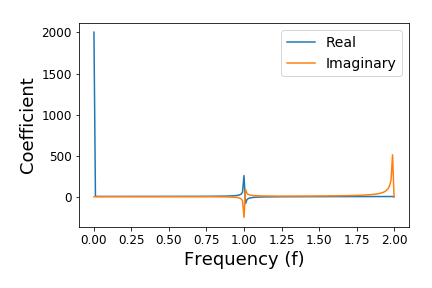
\includegraphics[width=\linewidth]{Coefficients}
\caption{The real and imaginary DFT coefficients at the range of frequencies detectable using the Nyquist frequency. Peaks occur in the expected three regions.}
\label{fig:Coefficients}
\end{figure}


\subsection{Power Spectrum and Filtering}
To investigate the properties of the power spectrum and the effects of
filtering, we consider the simple discretely sampled sinusoidal signal:
\begin{equation}
  V_j = A \sin(2 \pi f t_j - \phi)
  \label{eq:sine}
\end{equation}

As there is only one driving frequency in this function, it is expected that the power of the signal should be confined to a single frequency bin. This may be proven mathematically. To do so, it is sufficient to prove that the fourier transform of $V_j$ is confined to a single bin, since the power is merely the square of the Fourier amplitude in frequency space. This was done in equations \ref{eq:power}. Note that there were initially two peaks above, however for the DFT, our indices in frequency space, $k$, are only valid for positive $k$. Hence, the negative peak could be thrown out. The method was performed using a different valid definition for the DFT using a factor of $1/\sqrt{N}$ in both the forward and reverse transforms. Unfortunately, the proof above was off by a factor of $1/2$ that was not able to be reconciled. It it thought that this may due to removing the peak at a negative frequency. If the power from the negative peak was added to the positive instead of simply being removed, this would resolve the error.


\begin{equation}
\begin{split}
  V_j =& A \sin(2 \pi f t_j - \phi) \\
  V_j =& A \sin(2 \pi f (t_j -\frac{\phi}{2\pi f})) \\
  V_j =& A \sin(2 \pi f t'_j) \\
  \hat{V}_k =& \frac{1}{\sqrt{N}}\sum_{j=0}^{N-1} A\sin(2 \pi f t'_j) e^{-i2\pi kj/N} \\
  \hat{V}_k =& \frac{1}{\sqrt{N}}\sum_{j=0}^{N-1} \frac{A}{2i} (e^{2 \pi if t'_j} - e^{-2 \pi if t'_j}) e^{-i2\pi kj/N} \\
  \hat{V}_k =& \frac{1}{\sqrt{N}}\sum_{j=0}^{N-1} \frac{A}{2i} (e^{2 \pi i\Delta f k \Delta t' j} - e^{-2 \pi i\Delta f k \Delta t' j})\\
  & \quad \times e^{-i2\pi kj/N} \\
  let \quad k' =& \Delta f k \Delta t'N \\
  \hat{V}_k =& \frac{1}{\sqrt{N}}\sum_{j=0}^{N-1} \frac{A}{2i} (e^{\frac{2 \pi ij}{N} k'} - e^{-\frac{2 \pi ij}{N} k'}) e^{-i2\pi kj/N} \\
  \hat{V}_k =& \frac{1}{\sqrt{N}}\sum_{j=0}^{N-1} \frac{A}{2i} (e^{\frac{2 \pi ij}{N} (k' - k)} - e^{-\frac{2 \pi ij}{N} (k' + k)}) \\
  \hat{V}_k =& \frac{A\sqrt{N}}{2i} (\delta_{-k, k'} - \delta_{k,k'}) \\
  \hat{V}_k =& -\frac{A\sqrt{N}}{2i} \delta_{k,k'} \\
  P =& \hat{V}^* \hat{V} \\
  P =& \frac{A\sqrt{N}}{2i}\times -\frac{A\sqrt{N}}{2i} \\
  P =& \frac{A^2 N}{4}
\end{split}
\label{eq:power}
\end{equation}

\subsubsection{Power Spectra}
The power spectrum of a continuous signal is simply the square of the continuous
Fourier transform. However, when computing the power spectrum of a discretely
sampled signal, the leakage of power from some frequencies to others is a
problematic result of the digitization of the signal. To illustrate this, the
power spectra for two slightly different frequencies are considered: $f = 60$Hz
and $f = 59.673$Hz. These are shown in figure \ref{fig:power_spectra}. For the $60Hz$ peak, the power in the $60Hz$ bin is $5112\mu V^2$ and for the other frequency, $6088\mu V^2$. These values do not match the expected formula for the single bin. However, while the peaks are sharp in the plots, they are not confined to one bin. Importantly, if we add together the power for the whole spectrum, we get a value of $12500 \mu V^2$ in both cases, which matches the result obtained using the formula. Clearly there is some spectral leakage. To quantify the leakage, the total power in the 20 bins centered on the frequency of interest were examined. For $60Hz$ the power in these bins was $6142 \mu V^2$ and the power in $59.673$ was $6210\mu V^2$, indicating that the second frequency experienced more leakage.

\begin{figure}
  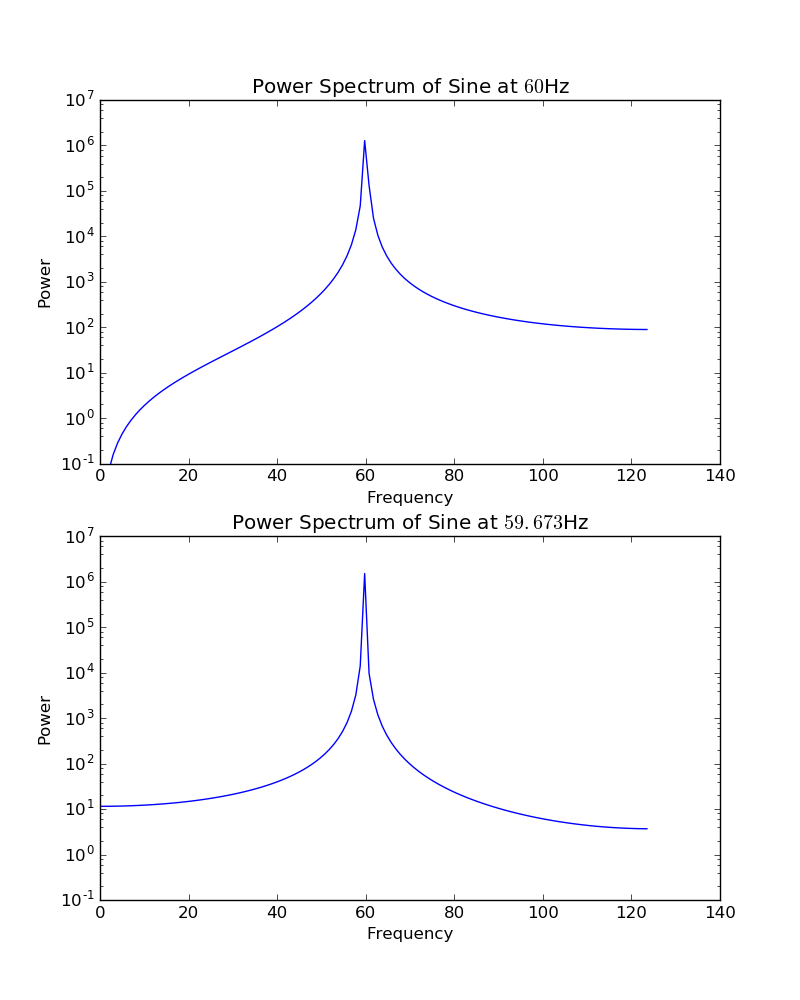
\includegraphics[width=\linewidth]{power_spectrum.png}
  \caption{
    The power spectra of equation \ref{eq:sine} with two very close
    frequencies. The top used a sine wave at $60Hz$ and the bottom at $59.673Hz$. These signals were generated with $250$ samples with
    a sampling rate of $125$Hz.
  }
  \label{fig:power_spectra}
\end{figure}

\subsubsection{Windows}
One of the standard ways to reduce spectral leakage is to multiply the data in
time space with a window before performing the Fourier transform. The
window should be equal to zero outside of the desired interval, thus
creating a window where the signal exists. All discretely sampled
signals can be thought of as having a rectangular window from when
sampling began to the most recent measurement. Two of the
most common windows we look into are the Hann window and the Blackman-Harris
window. The Hann function and its Fourier transform are shown in figure
\ref{fig:hann_window}. In time space, it is akin to applying part of a
cosine wave to the signal. In frequency space, however, it can be
interpreted as applying a convolution to Fourier transform of the
signal. 

\begin{figure}[t]
  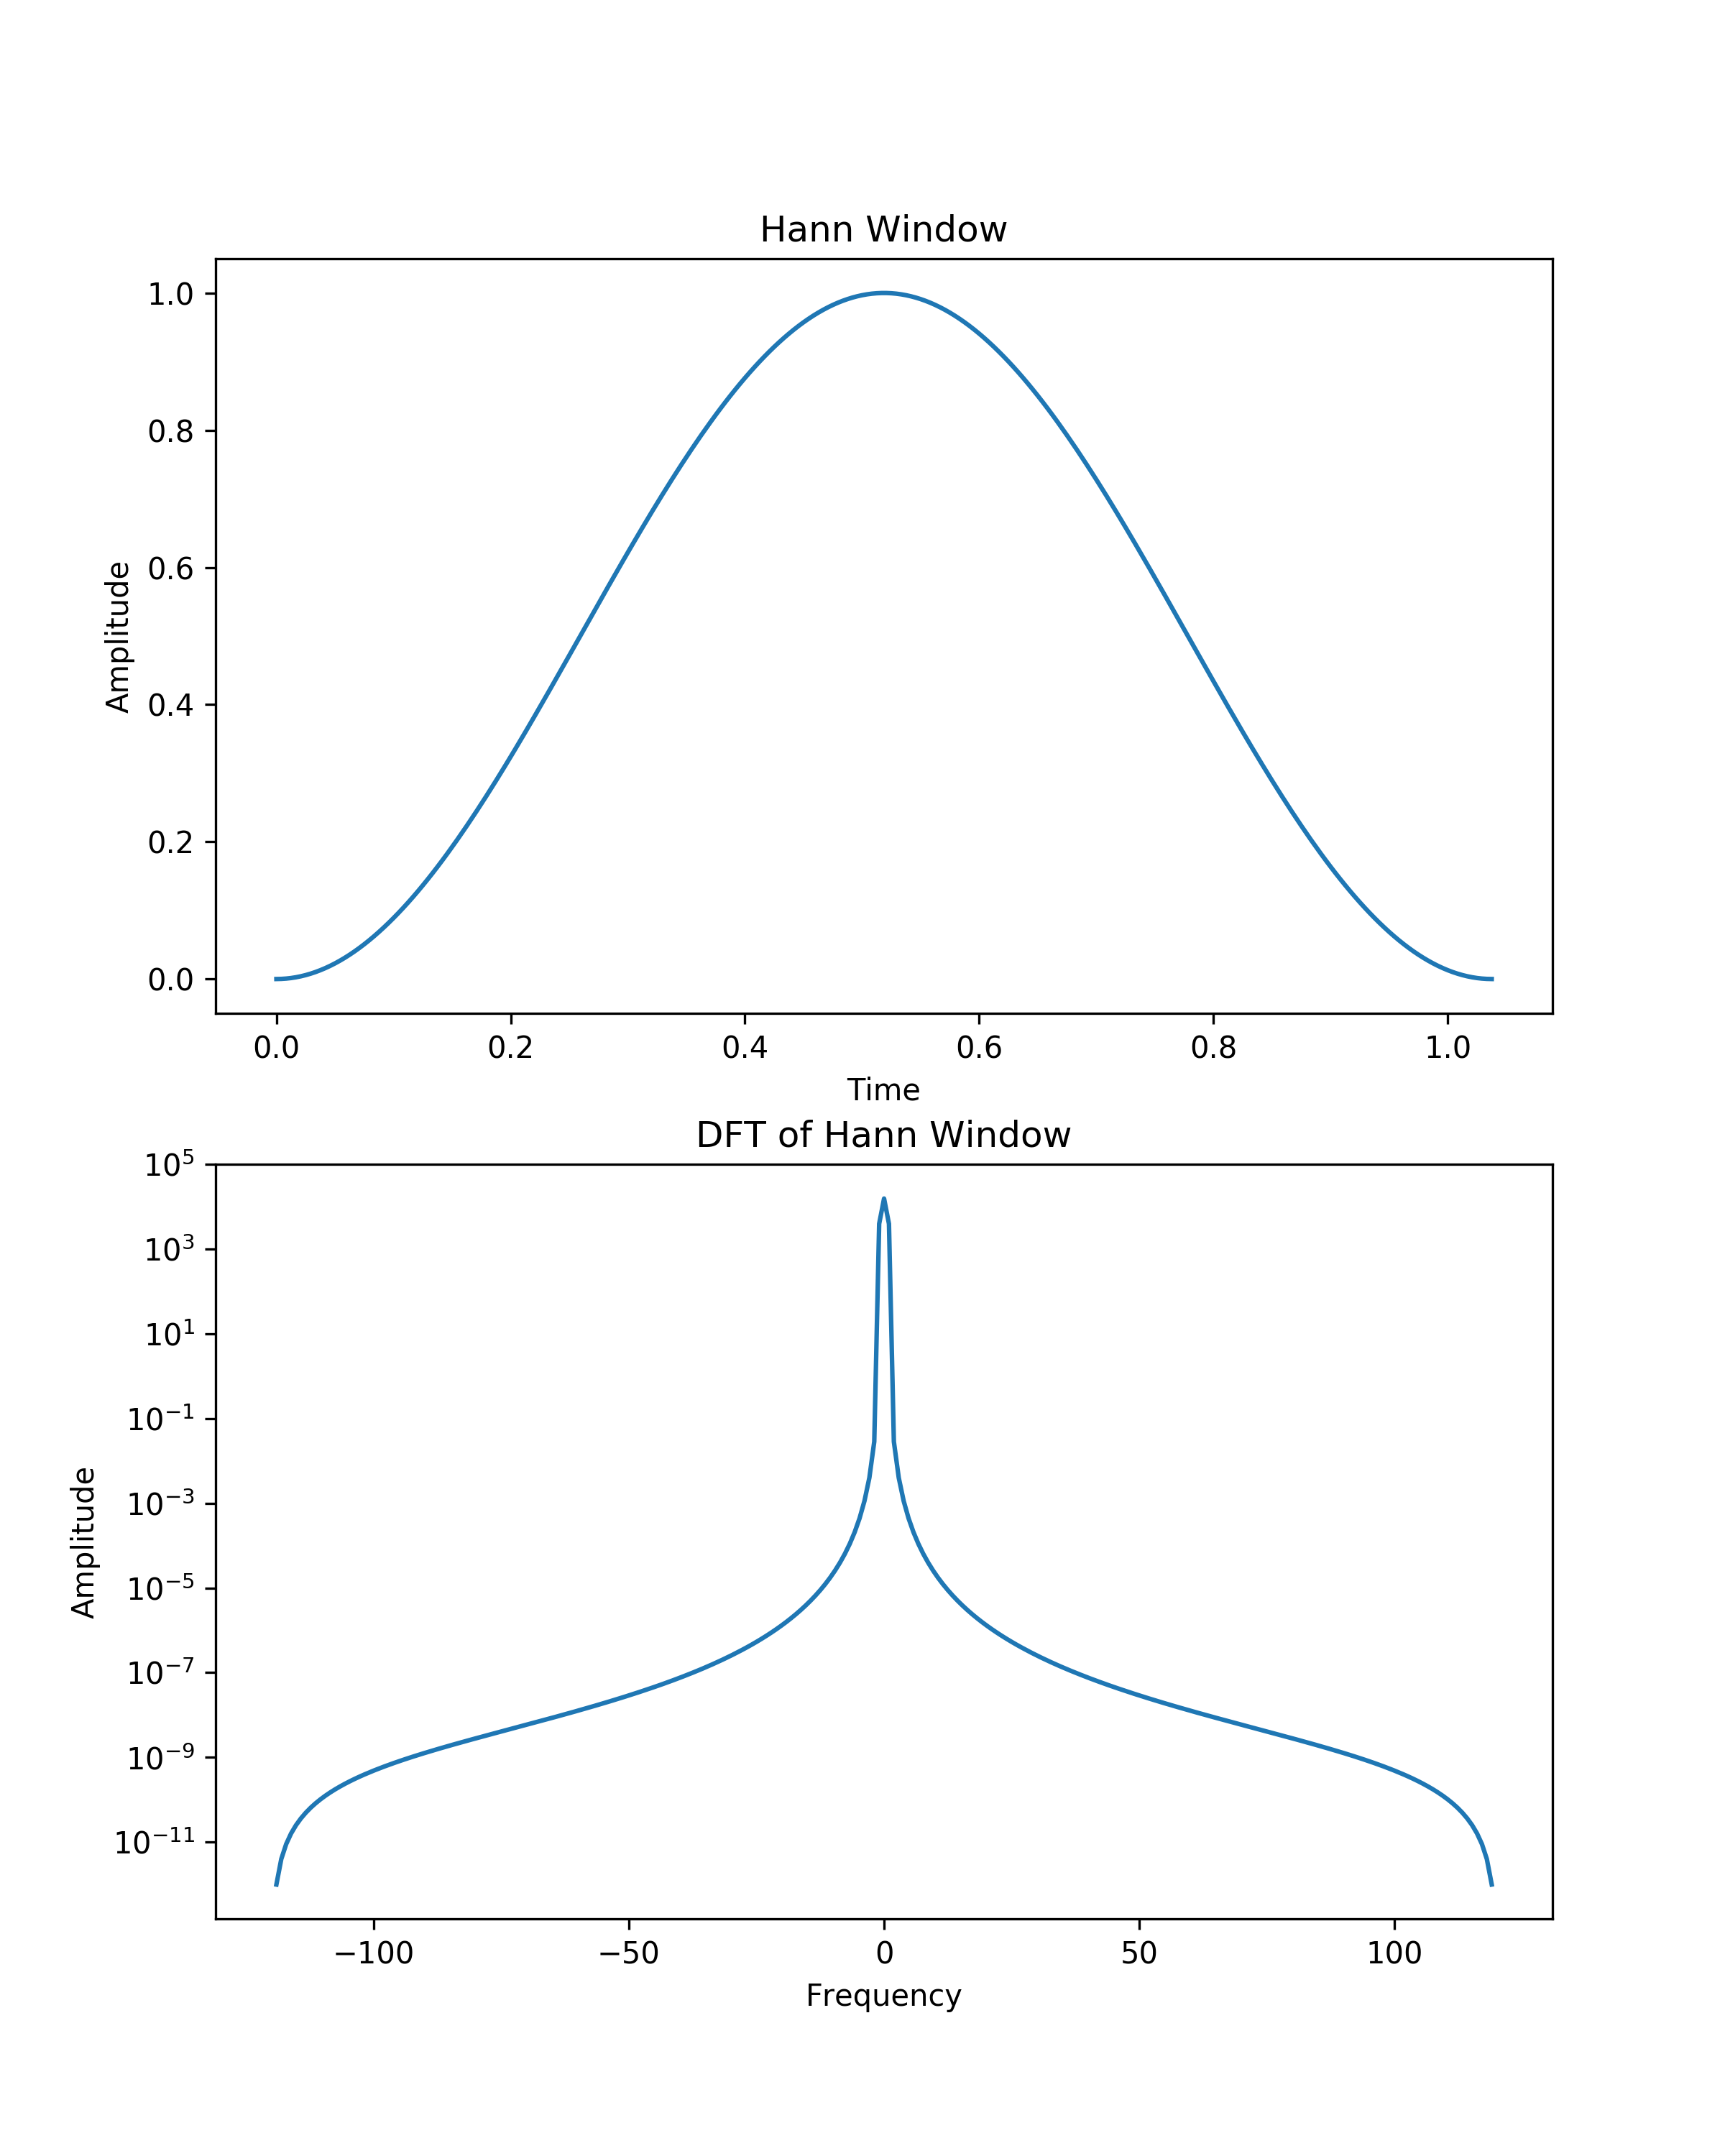
\includegraphics[width=\linewidth]{hann_window.png}
  \caption{
    The Hann window (top) and its Fourier transform (bottom). It can be thought
    of as a portion of a cosine wave.
  }
  \label{fig:hann_window}
\end{figure}

Now the Hann window can be applied to the two signals that were used previously
with frequencies $60$Hz and $59.673$Hz, shown in figures \ref{fig:hann_0} and
\ref{fig:hann_1}, respectively. The windowed function, shown in the
top panel of figure \ref{fig:hann_0}, now has an envelope, but there are also smaller beats that
appear to emerge which are not actually in the signal. This is
reflected in the power spectrum, shown in the lower panel, where the
peak has broadened the peak but has also decreased the power for the
higher frequencies. These similar effects can also be seen in figure
\ref{fig:hann_1} for the frequency $f = 59.673$, though the
higher frequencies reduced even further.

\begin{figure}[t]
  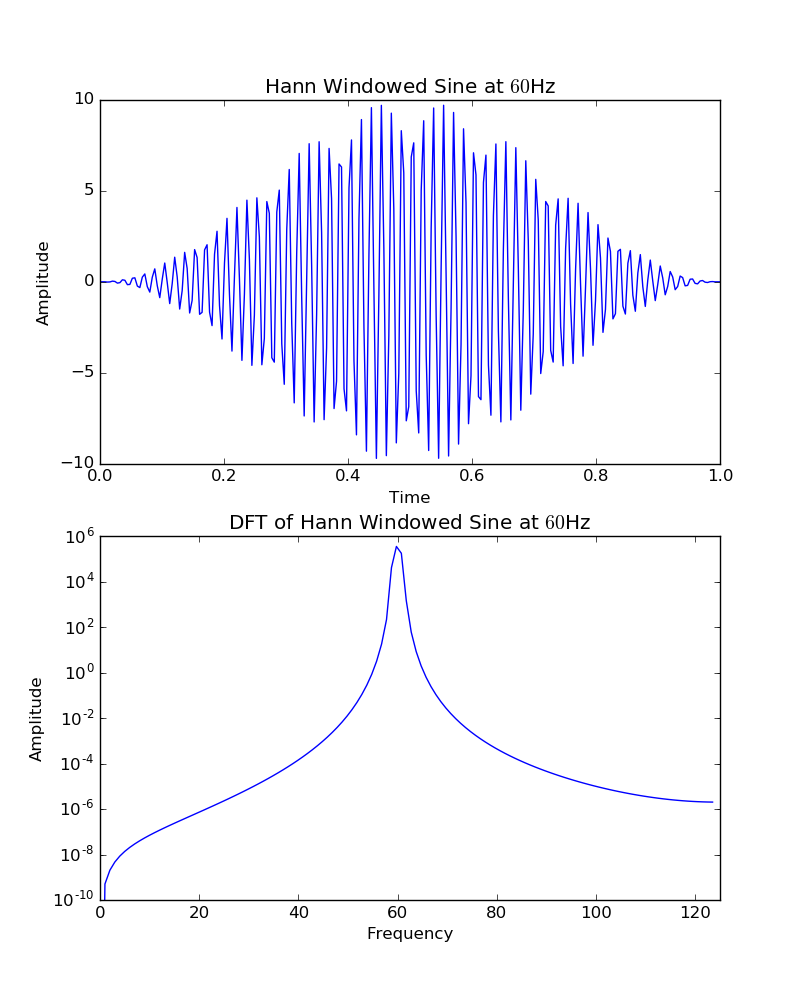
\includegraphics[width=\linewidth]{hann_0.png}
  \caption{
    The Hann window applied to equation \ref{eq:sine} with $f = 60$Hz in time
    space (top) and in frequency space (bottom).
  }
  \label{fig:hann_0}
\end{figure}

\begin{figure}[t]
  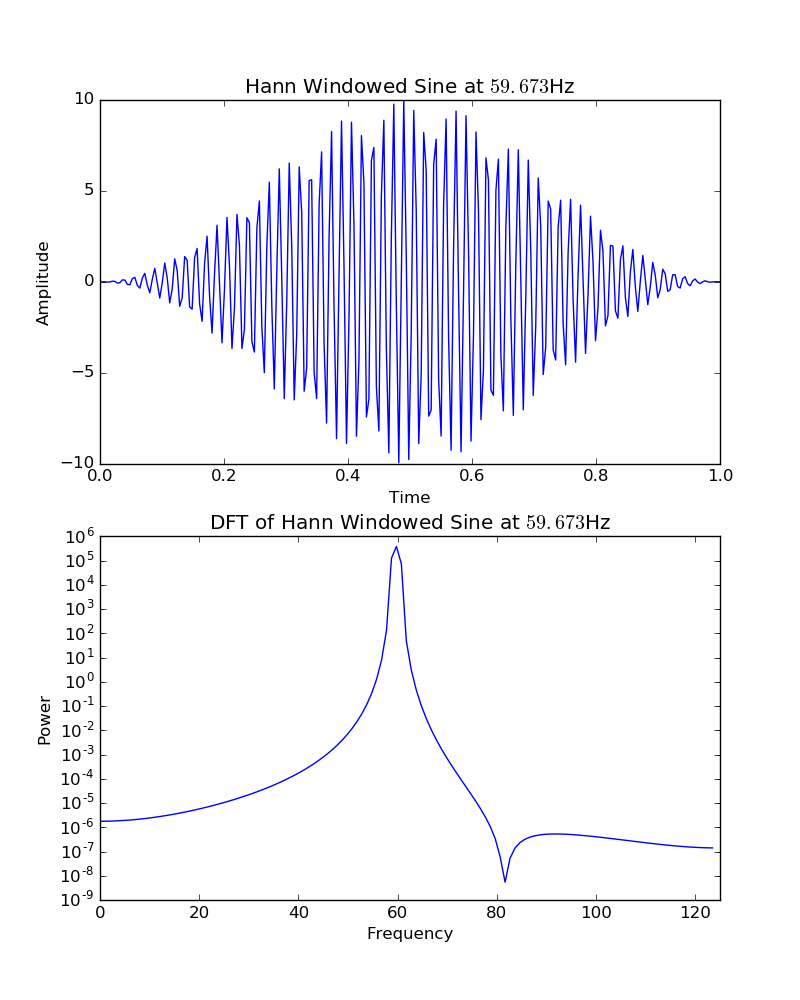
\includegraphics[width=\linewidth]{hann_1.png}
  \caption{
    The Hann window applied to equation \ref{eq:sine} with $f = 59.673$Hz in
    time space (top) and in frequency space (bottom).
  }
  \label{fig:hann_1}
\end{figure}

We can compare the results of using the Hann window with the
Blackman-Harris window, shown in figure \ref{fig:blackman_harris}. The Fourier transform of the Blackman-Harris
window has a very distinct local minima around the peak. When this is
applied to the signal, the peaks at $60$Hz also have distinct minima
around them. However, this also widens the peak and decreases the
power of the surrounding frequencies.

\begin{figure*}
  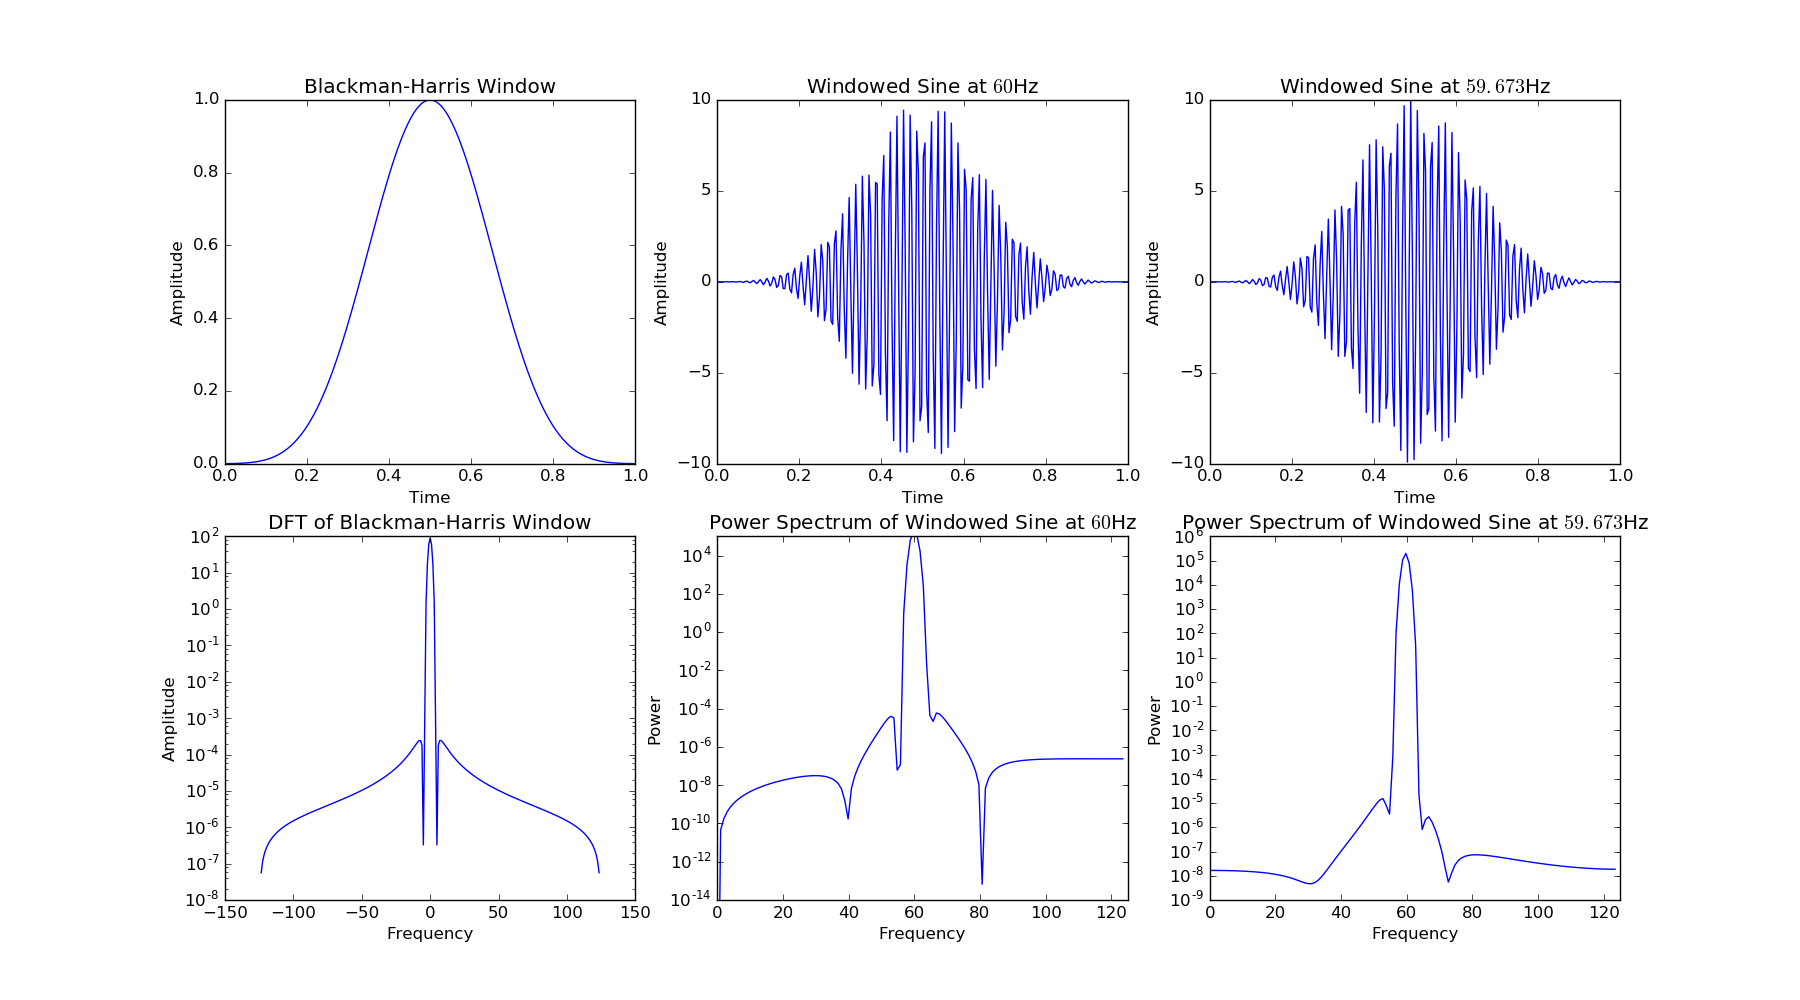
\includegraphics[width=\linewidth]{blackman_harris.png}
  \caption{
    The Blackman-Harris window is also applied to the sine wave with
    frequencies $f = 60$Hz and $f = 69.673$Hz. The functions in time space are
    shown in the top row while the bottom row shows the Fourier transform of the
    Blackman-Harris window and the power spectra of the functions above.
  }
  \label{fig:blackman_harris}
\end{figure*}


\section{Applications}
\subsection{Stellar Binary System}

Stellar binary stars are pairs of stars that orbit each other. As the stars are far away, it may be difficult for the naked eye or even a telescope to see two separate objects due to the overlapping point spread functions of the two stars. In order to detect such systems, a property of the stars' orbit may be used. For most planes of viewing, one star will pass in front of the other star, partially obscuring it and changing the intensity of light reaching a telescope. By examining star intensity as a function of time, binary systems may be isolated, as this section will show.

A set of data were provided describing photon count rate coming from a combination of a pulsar and another star. Figure \ref{fig:binary_time} shows the time series of the data. Due to the size of the data set, periodicities were difficult to spot in the light curve. First, a Fourier transform was applied to the data to analyse the signal. Because there was also interest in the region close to $f=0$, the FFT figure was discarded in favor of a Lomb-Scargle algorithm. The chi-squared implementation was used from the astropy library. Figure \ref{fig:BinarySpectrum} shows the Lomb-Scargle power spectrum of the data. A series of five prominent peaks at values around $0.9Hz$, $1.6Hz$, $2.3Hz$, $3.2Hz$ and $4.0Hz$ shows that the system is indeed periodic. There are a number of smaller peaks in these regions as well. Where the main peaks were so large, the data were also examined between the peaks for smaller peaks that may have been obscured by the choice of scaling. Figure \ref{fig:binaryZoom} shows the region around $f=0$. There are a few small peaks in this region corresponding to very low frequency signals. To test if these peaks were significant, the data was tested using astropy's \texttt{LombScargle.false\char`_alarm\char`_level()} function. This function returned the amplitude at which the peaks would exceed a given p-score. None of the peaks exceeded the threshold for $p=0.1$, suggesting that these peaks were not significant. 

\begin{figure*}
\centering
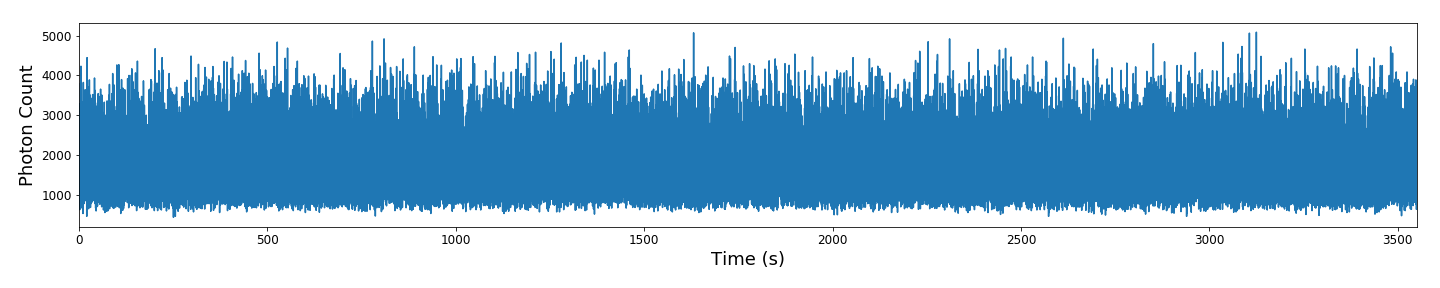
\includegraphics[width=\textwidth]{binary_time}
\caption{Time spectrum of a binary stellar system. Since any underlying periodicies are not immediately obvious in the time spectrum, the frequency spectrum will be required to determine any periodic effects.}
\label{fig:binary_time}
\end{figure*}

\begin{figure}
\centering
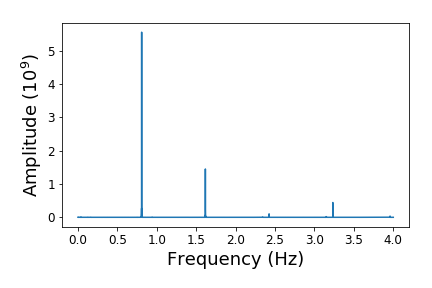
\includegraphics[width=\linewidth]{BinarySpectrum}
\caption{Frequency spectrum of a stellar binary system. The spectrum was determined using astropy's chi-squared implementation of the Lomb-Scargle method. There are a series of well defined peaks indicating periodic behaviour. Where the peaks are extremely high, there may be some peaks that are lost due to scaling.}
\label{fig:BinarySpectrum}
\end{figure}

\begin{figure}
\centering
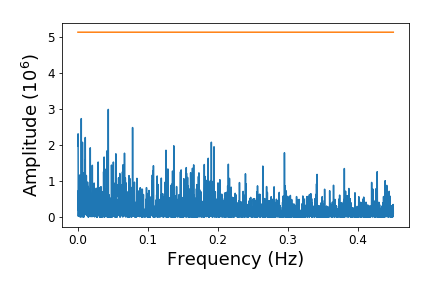
\includegraphics[width=\linewidth]{binaryZoom}
\caption{Close-up of figure \ref{fig:BinarySpectrum} near $f=0$. There are peaks in this region corresponding to very long periods. Applying a chi-squared test to the data however suggest that these peaks are not significant. The orange line indicates the threshold that a peak needs to exceed to have a p-score greater than $p=0.1$.}
\label{fig:binaryZoom}
\end{figure}

\subsection{Heart Beats}
The data gives a time sequence of heart beats sampled at $125$Hz. Since the data
is evenly sampled and the number of samples is a power of two, padding is not
necessary in this case. The amplitude spectrum is shown in figure
\ref{fig:beats}. The two most dominant frequencies are approximately $2$Hz and
$4$kHz, with corresponding periods $0.5$s and $0.25$s, respectively.

\begin{figure}
  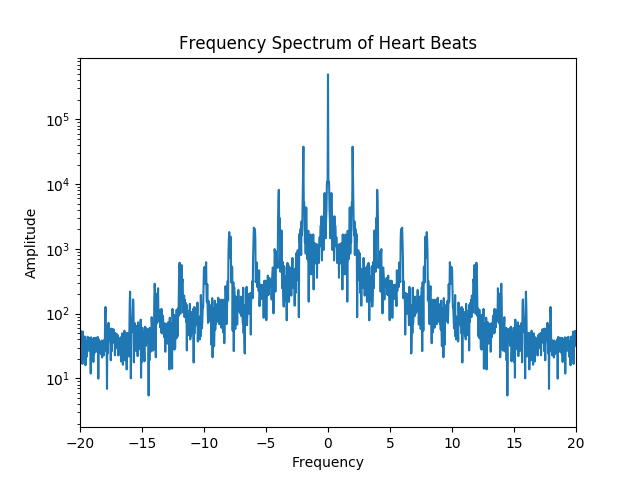
\includegraphics[width=\linewidth]{beats.png}
  \caption{
    The amplitude spectrum of the patient's heart beats. The data was sampled at
    $125$Hz and has $4096$ samples.
  }
  \label{fig:beats}
\end{figure}

The average resting heart rate is about $60$ to $100$ beats per minute. However,
this translates to periods within a range of $1$s to $1.6$s, which are
significantly faster than that of the patient. This would suggest that the
patient was not at rest before the measurement or some other reason for a faster
heart rate. The $2$Hz heart rate can be explained through the patient
exercising or a medical condition. However, the heart rate of $4$Hz,
or $240$ beats per minute, is much more unrealistic. There are peaks
that occur periodically as the frequency axis increases, and may be an
artifact of sampling.

\subsection{Solar Activity}
Sunspots are a feature of the sun that correspond to its magnetic properties and temperature. A datafile was provided that recorded the number of sunspots visible in a given month. As usual, the data were first plotted to gain an intuitive look at the data.

\begin{figure*}
\centering
\includegraphics[width=\textwidth]{"sunspot time"}
\caption{Time spectrum of number of sunspots visible on the sun. A clear periodic pattern is visible. This behaviour was estimated in the time spectrum by guessing a period and placing vertical dividers to test the fit of the periodicity until a value with a good fit was obtained. The best estimate was a period of $130$ months.}
\label{fig:sunspottime}
\end{figure*}

By looking at the data it was apparent that there was some sort of periodicity. This was determined by guessing the period and repeatedly plotting the start of a period according to this guess. Guesses were adjusted until the best possible fit was obtained. The best found guess was $130$ months. This guess was then tested by taking the power spectrum of the data. The power spectrum required taking a FFT of the data. Since the number of data points ($2141$) was not a power of 2, this data set needed to be padded with zeros to perform a FFT. Thankfully, the numpy \texttt{numpy.fft.fft} function automatically padded the zeros and used efficient algorithms to minimize the padding needed.  From this power data, the maximum peak occurred at a frequency corresponding to $T=130.875$ months. This was extremely close to the guess, and corresponds to a period of almost exactly 11 years.

\begin{figure}
\centering
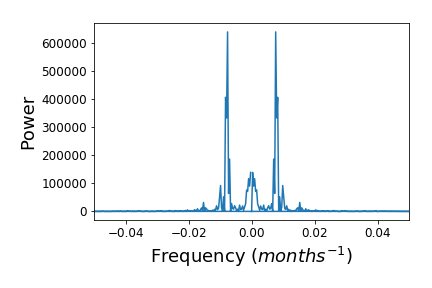
\includegraphics[width=\linewidth]{SunSpotPowerSpectrum}
\caption{Power spectrum of the sunspot time series in figure \ref{fig:sunspottime}. The spectrum has been cropped to the only region with large peaks around $f=0$.}
\label{fig:SunSpotPowerSpectrum}
\end{figure}

\subsection{Financial Series}
For this section, we analyze the stock prices for 6 companies, shown in figure
\ref{fig:stocks_time}.

\begin{figure}
  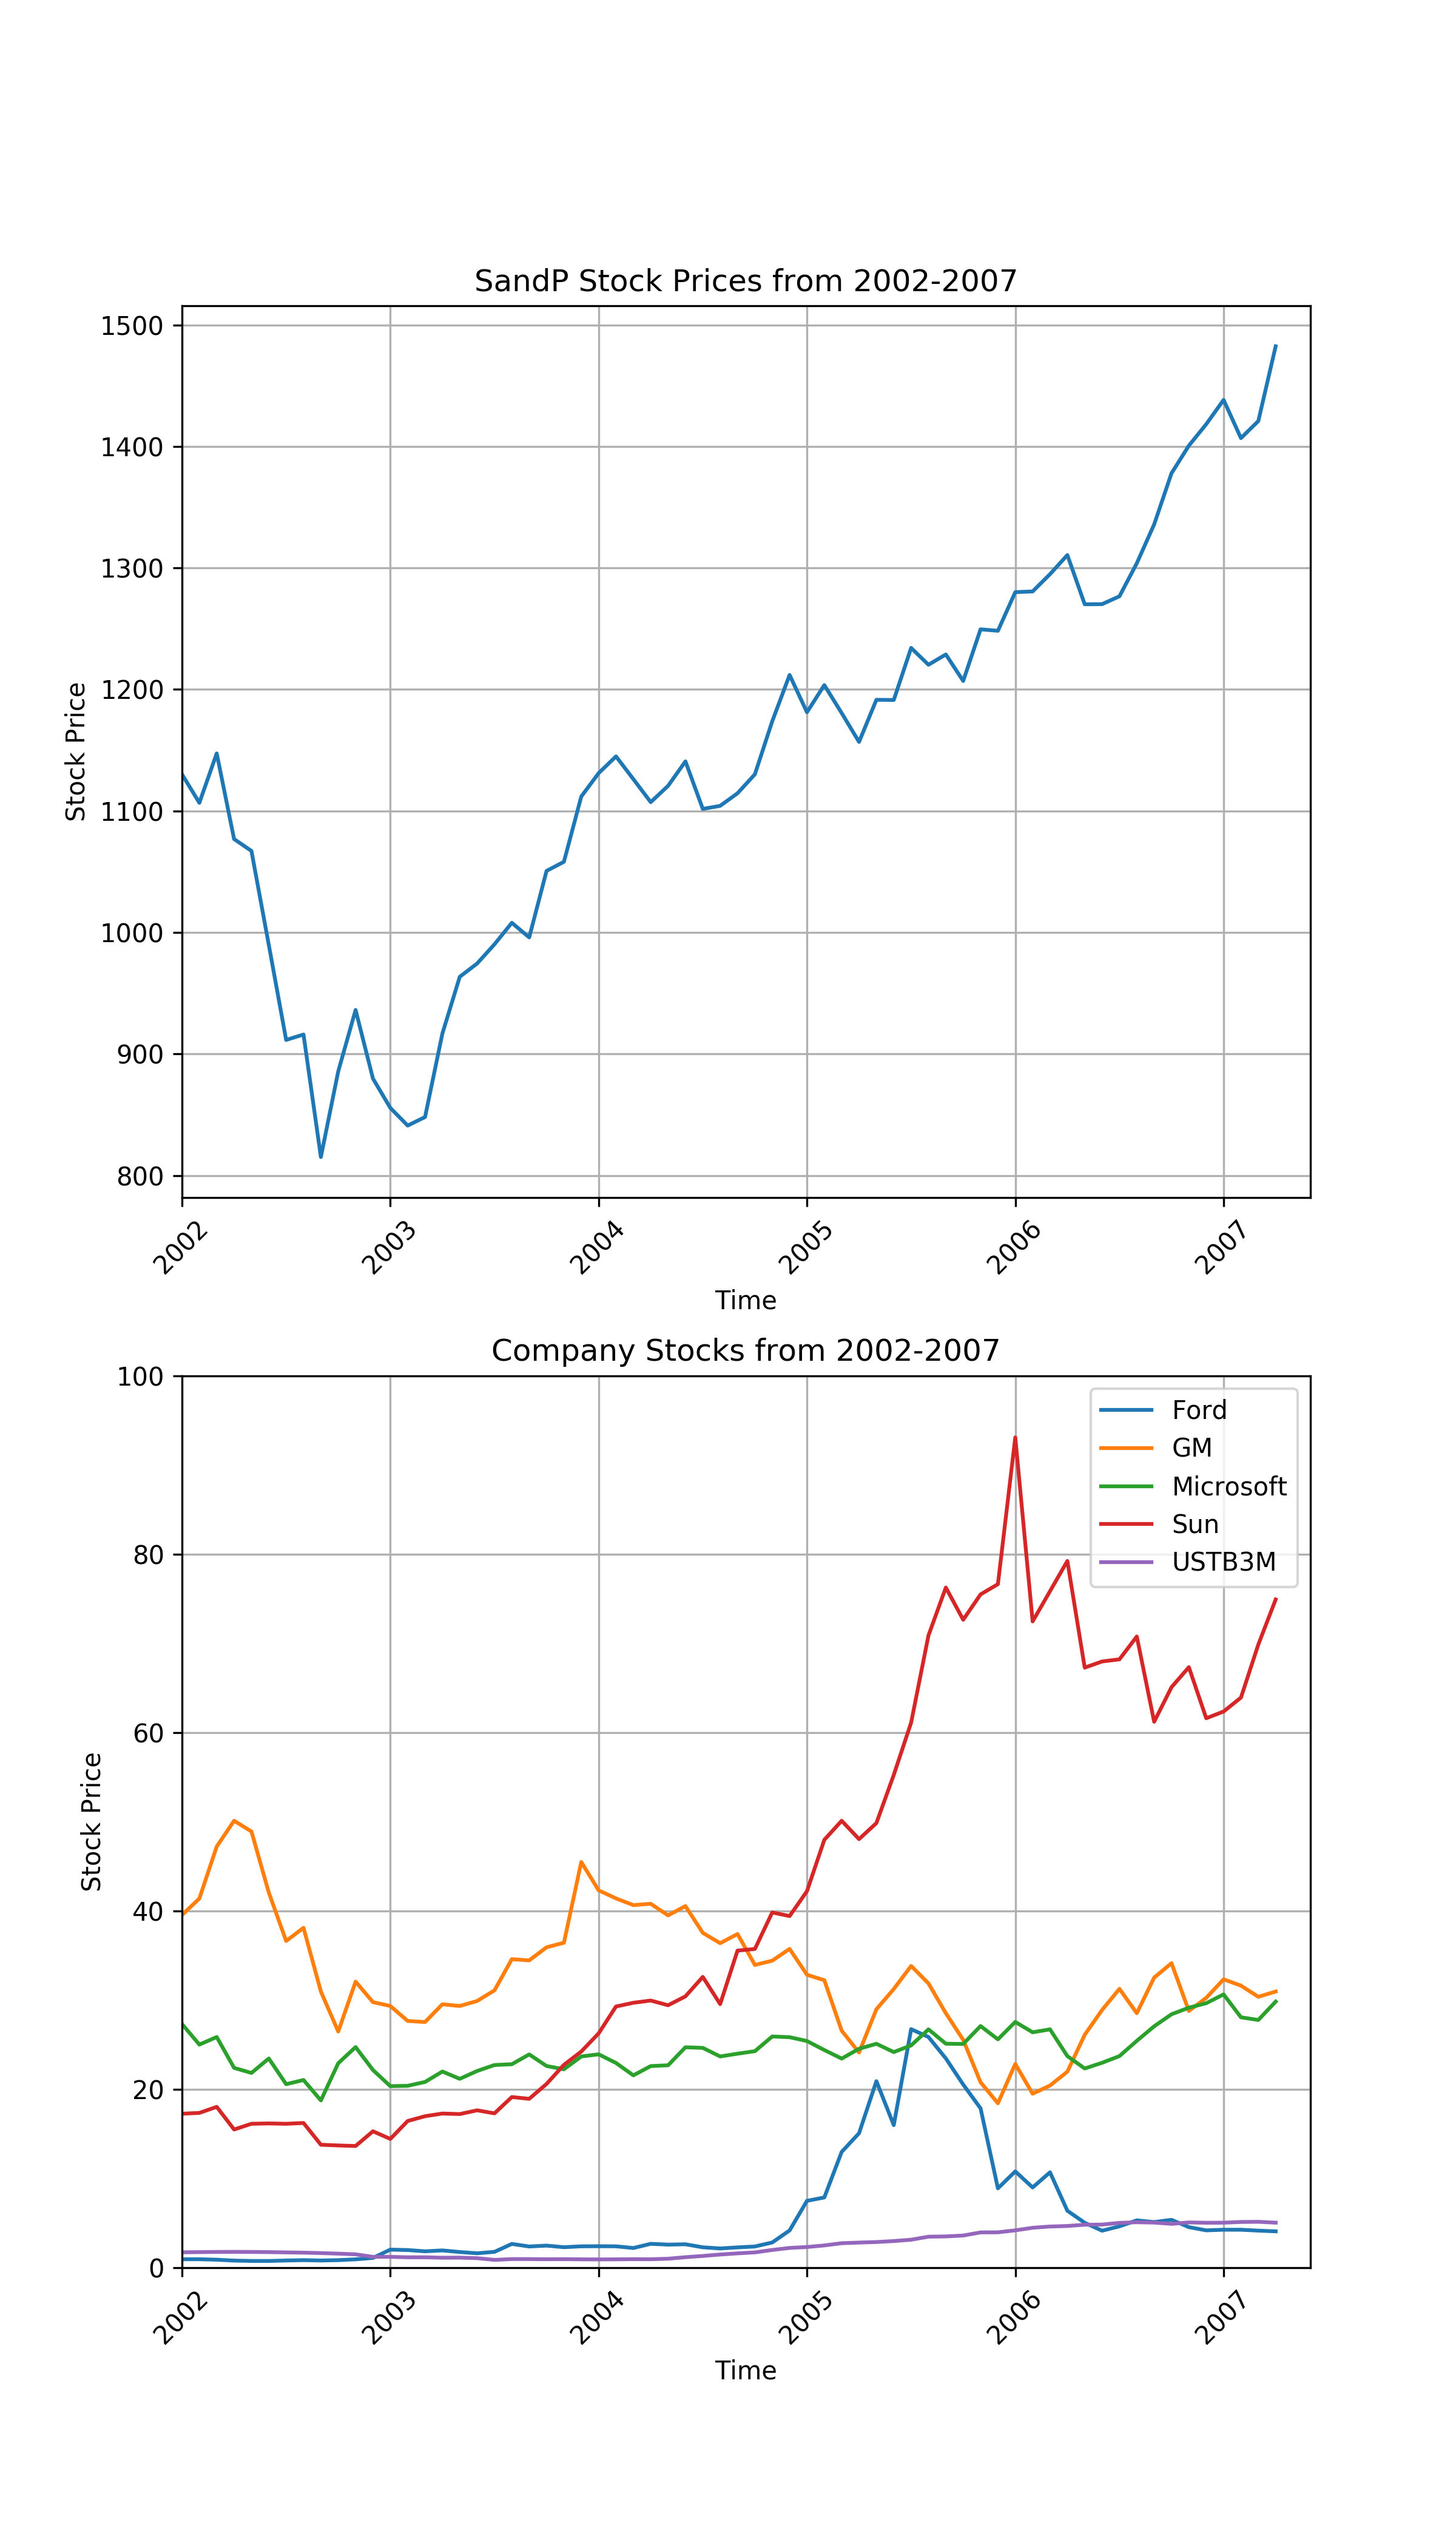
\includegraphics[width=\linewidth]{stocks_time.png}
  \caption{
    The monthly stock prices of six companies from $2002$ through to mid-$2007$.
  }
  \label{fig:stocks_time}
\end{figure}

This data is then used to compute the continuously compounded returns $R_i$,
given by the relation:
\begin{equation}
  R_i = \ln\left( \frac{P_i}{P_{i-1}} \right)
  \label{ccr}
\end{equation}
which are shown in figure \ref{fig:stocks_returns}. The autocorrelation of the
returns are shown in \ref{fig:stocks_ac}. The autocorrelation for all
of the companies oscillate around zero, meaning that the behaviour of
the returns is actually very random and cannot easily be predicted
based on the previous prices. This is a rather surprising result
because some of the graphs of the time series may appear to have clear
trends. The power spectra of the returns (figure \ref{fig:stocks_pc}
also show that the returns is composed of many different frequencies,
which indicates that the actual function is difficult to predict.

\begin{figure*}
  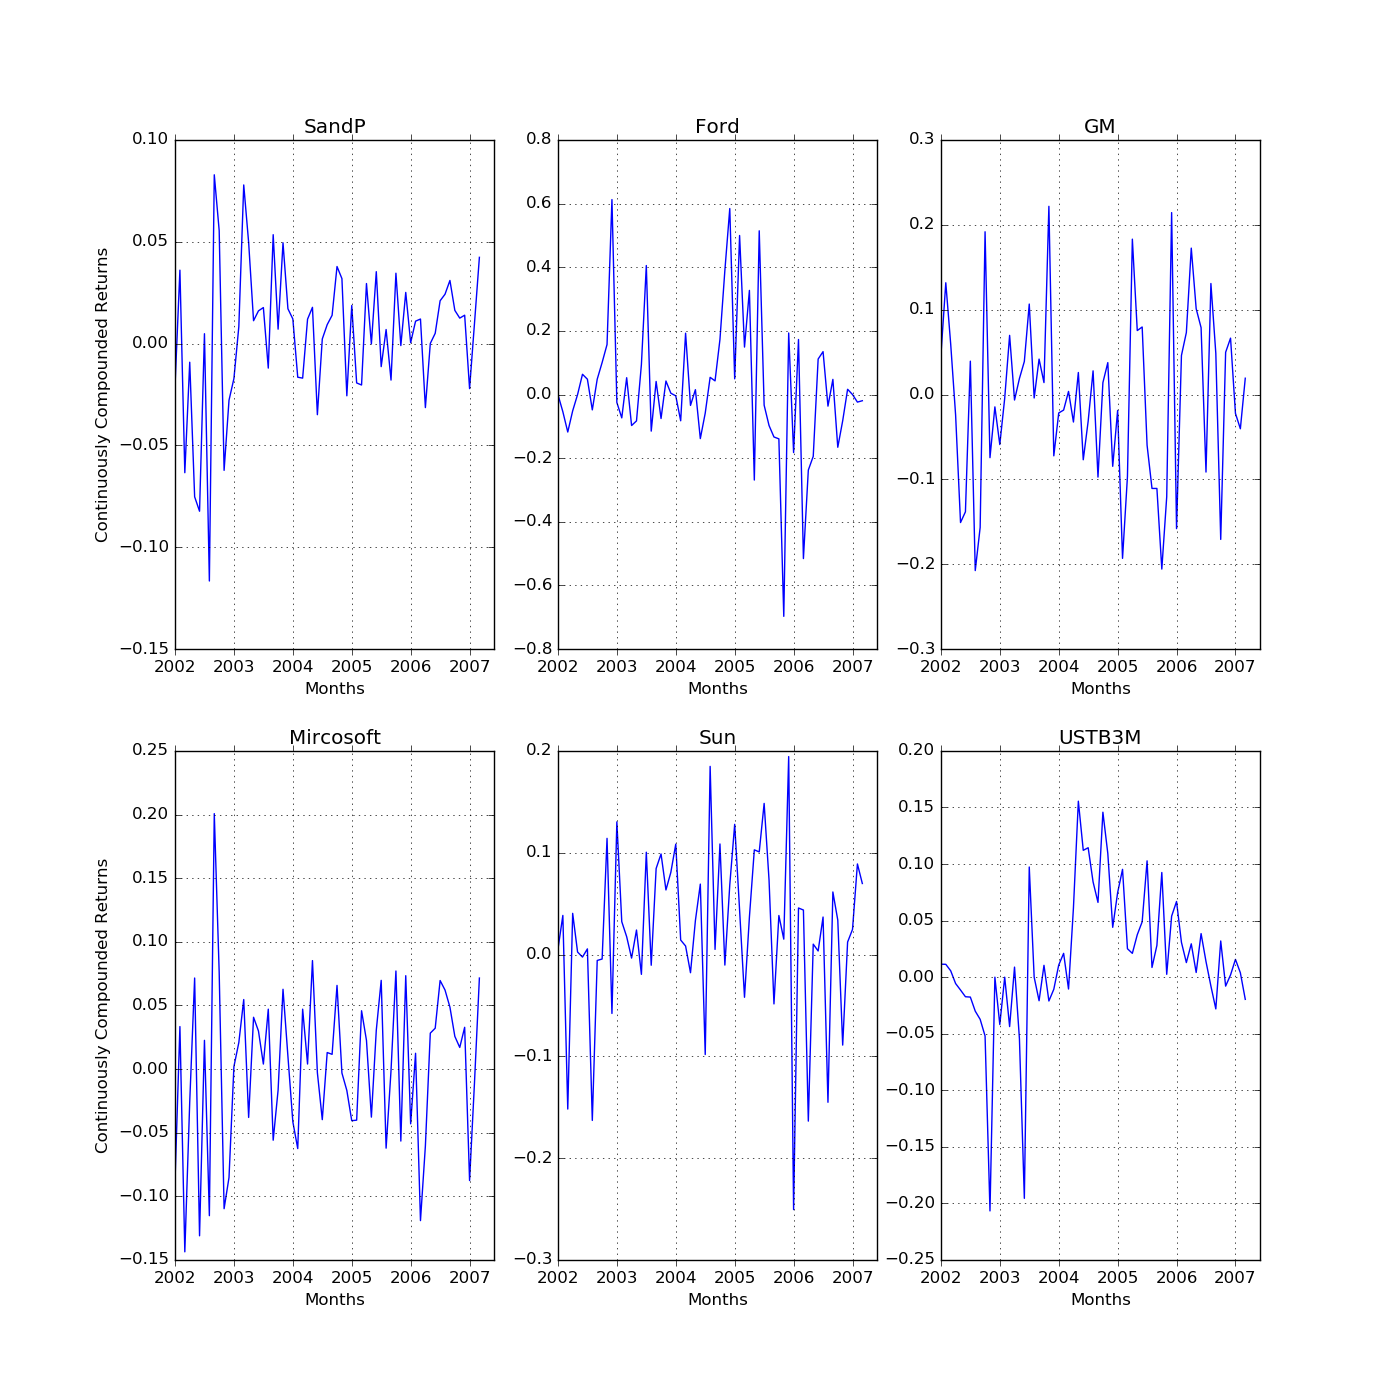
\includegraphics[width=\linewidth]{stocks_returns.png}
  \caption{
    The continuously compunded returns of six companies. The returns were
    computed from the data in figure \ref{fig:stocks_time} using equation
    \ref{ccr}.
  }
  \label{fig:stocks_returns}
\end{figure*}

\begin{figure*}
  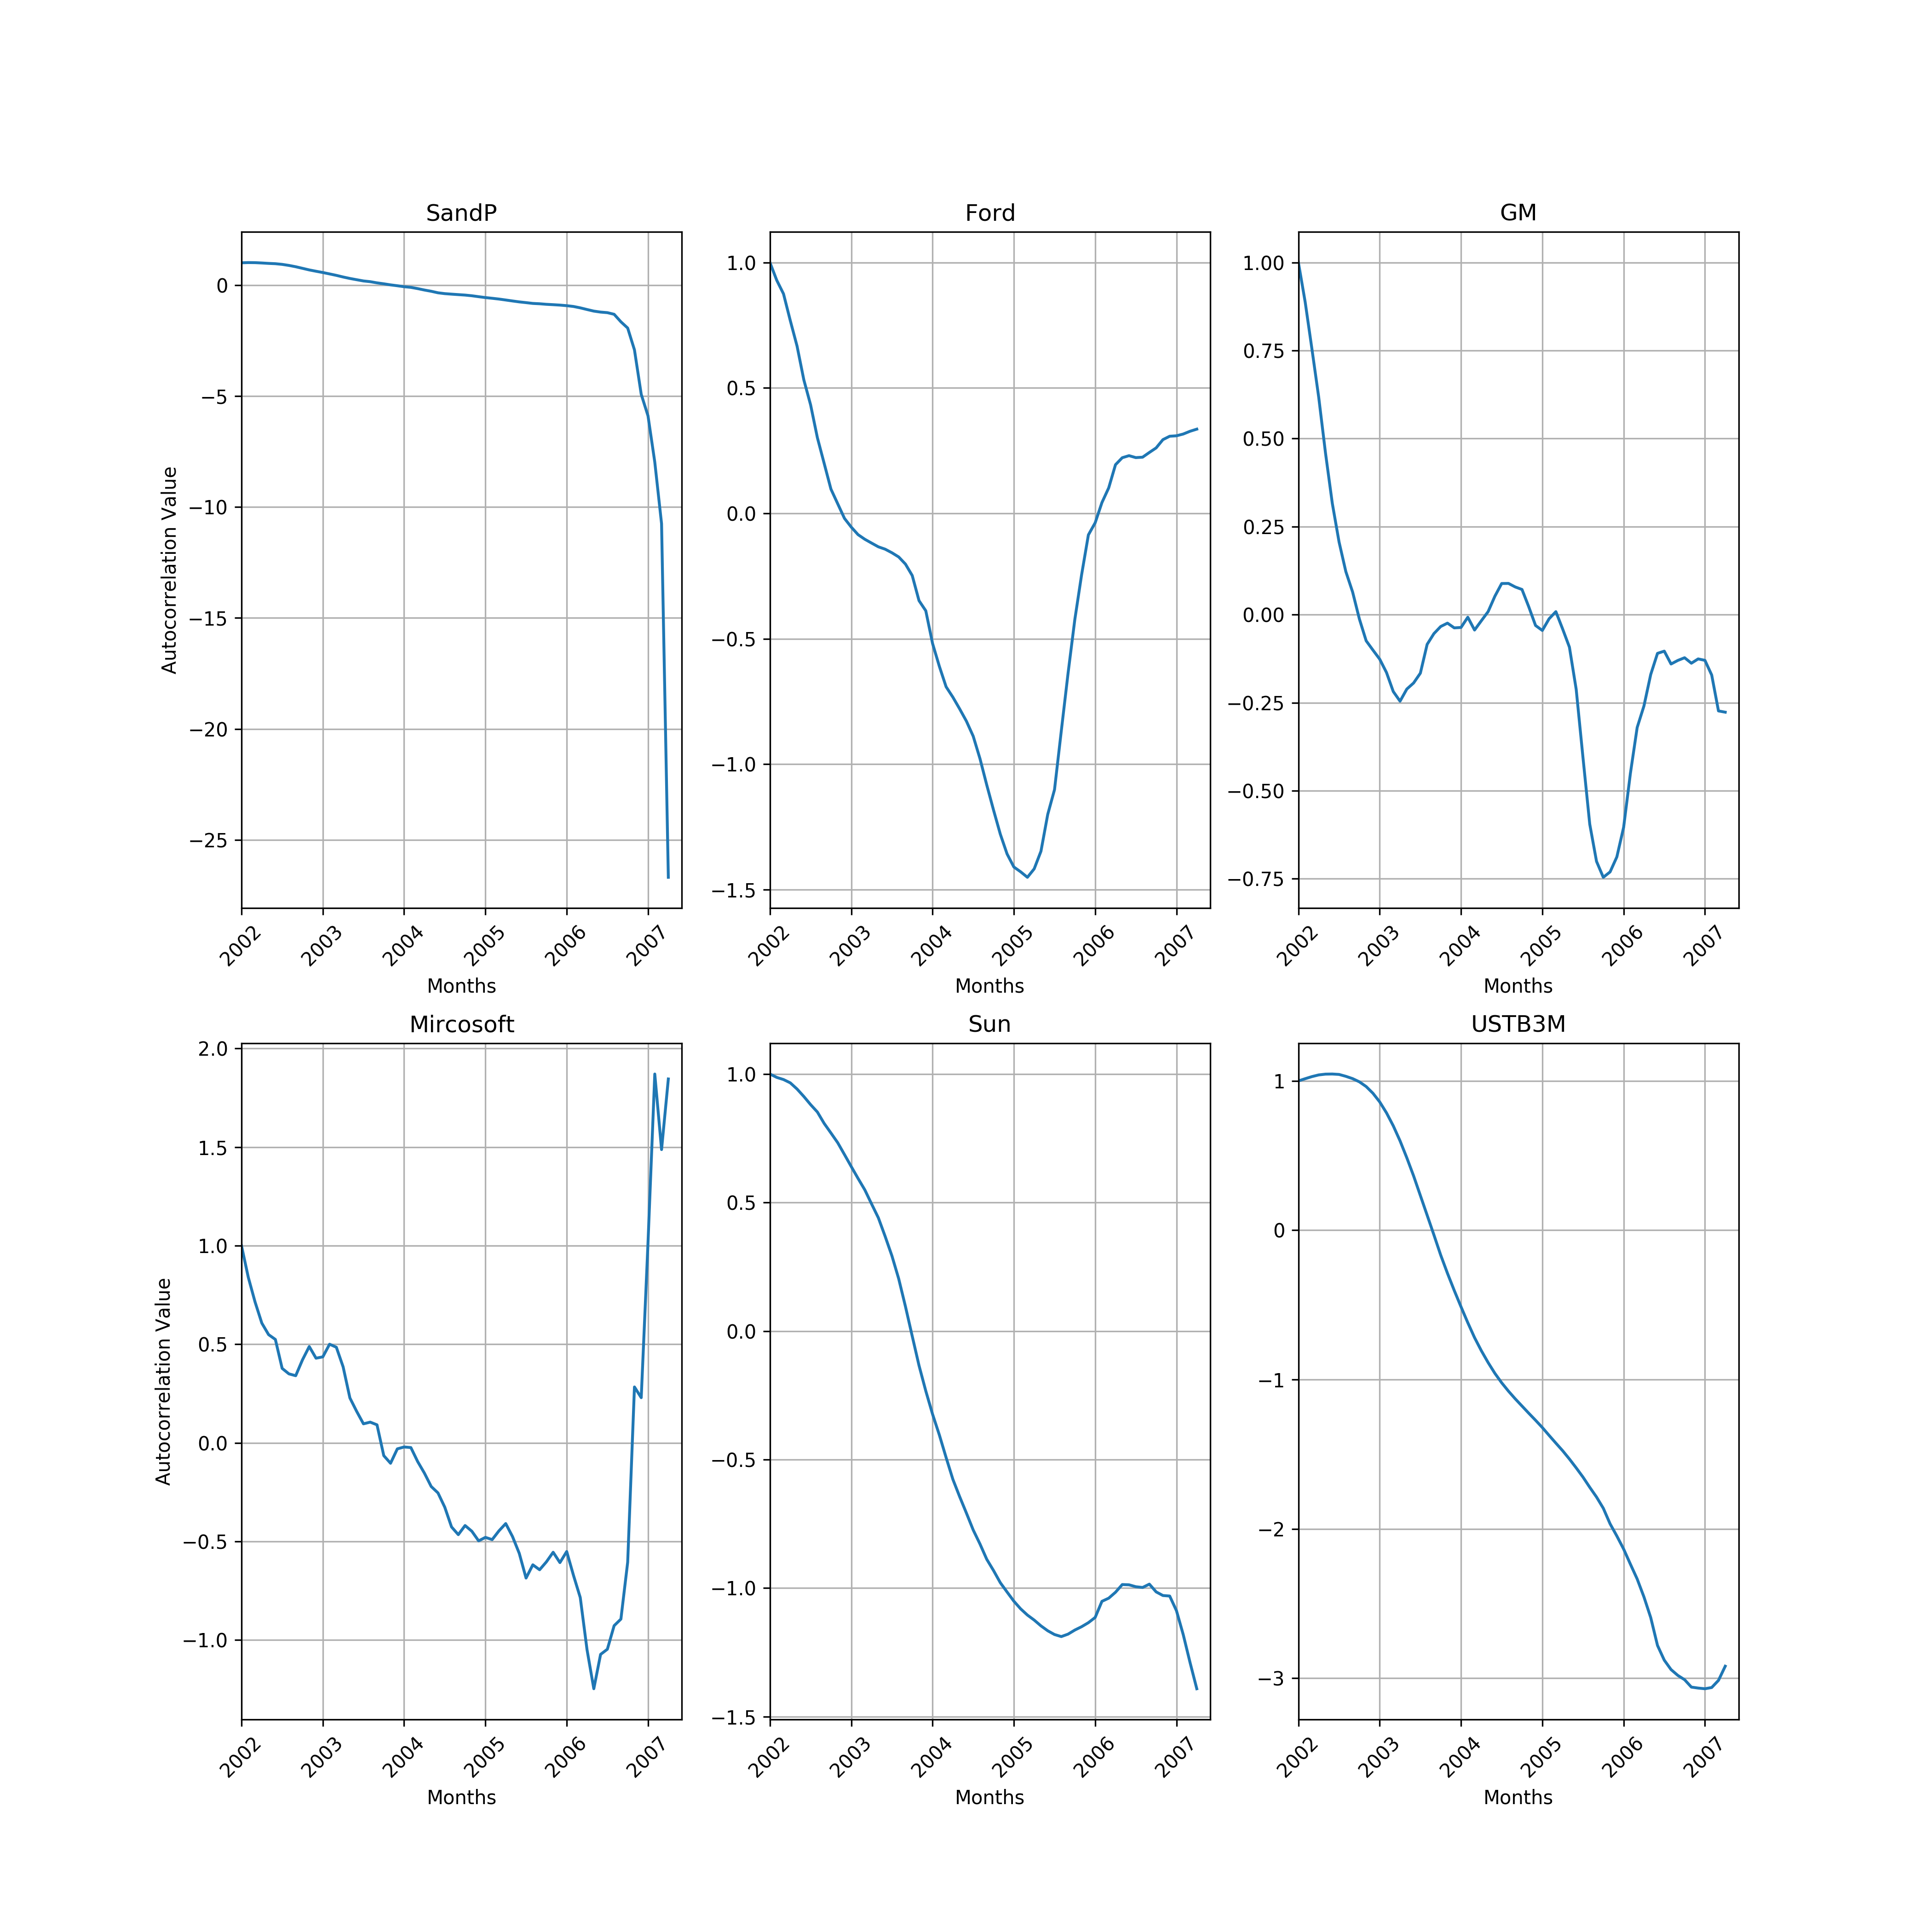
\includegraphics[width=\linewidth]{stocks_ac.png}
  \caption{
    The autocorrelation of the compounded returns of six companies.
  }
  \label{fig:stocks_ac}
\end{figure*}

\begin{figure*}
  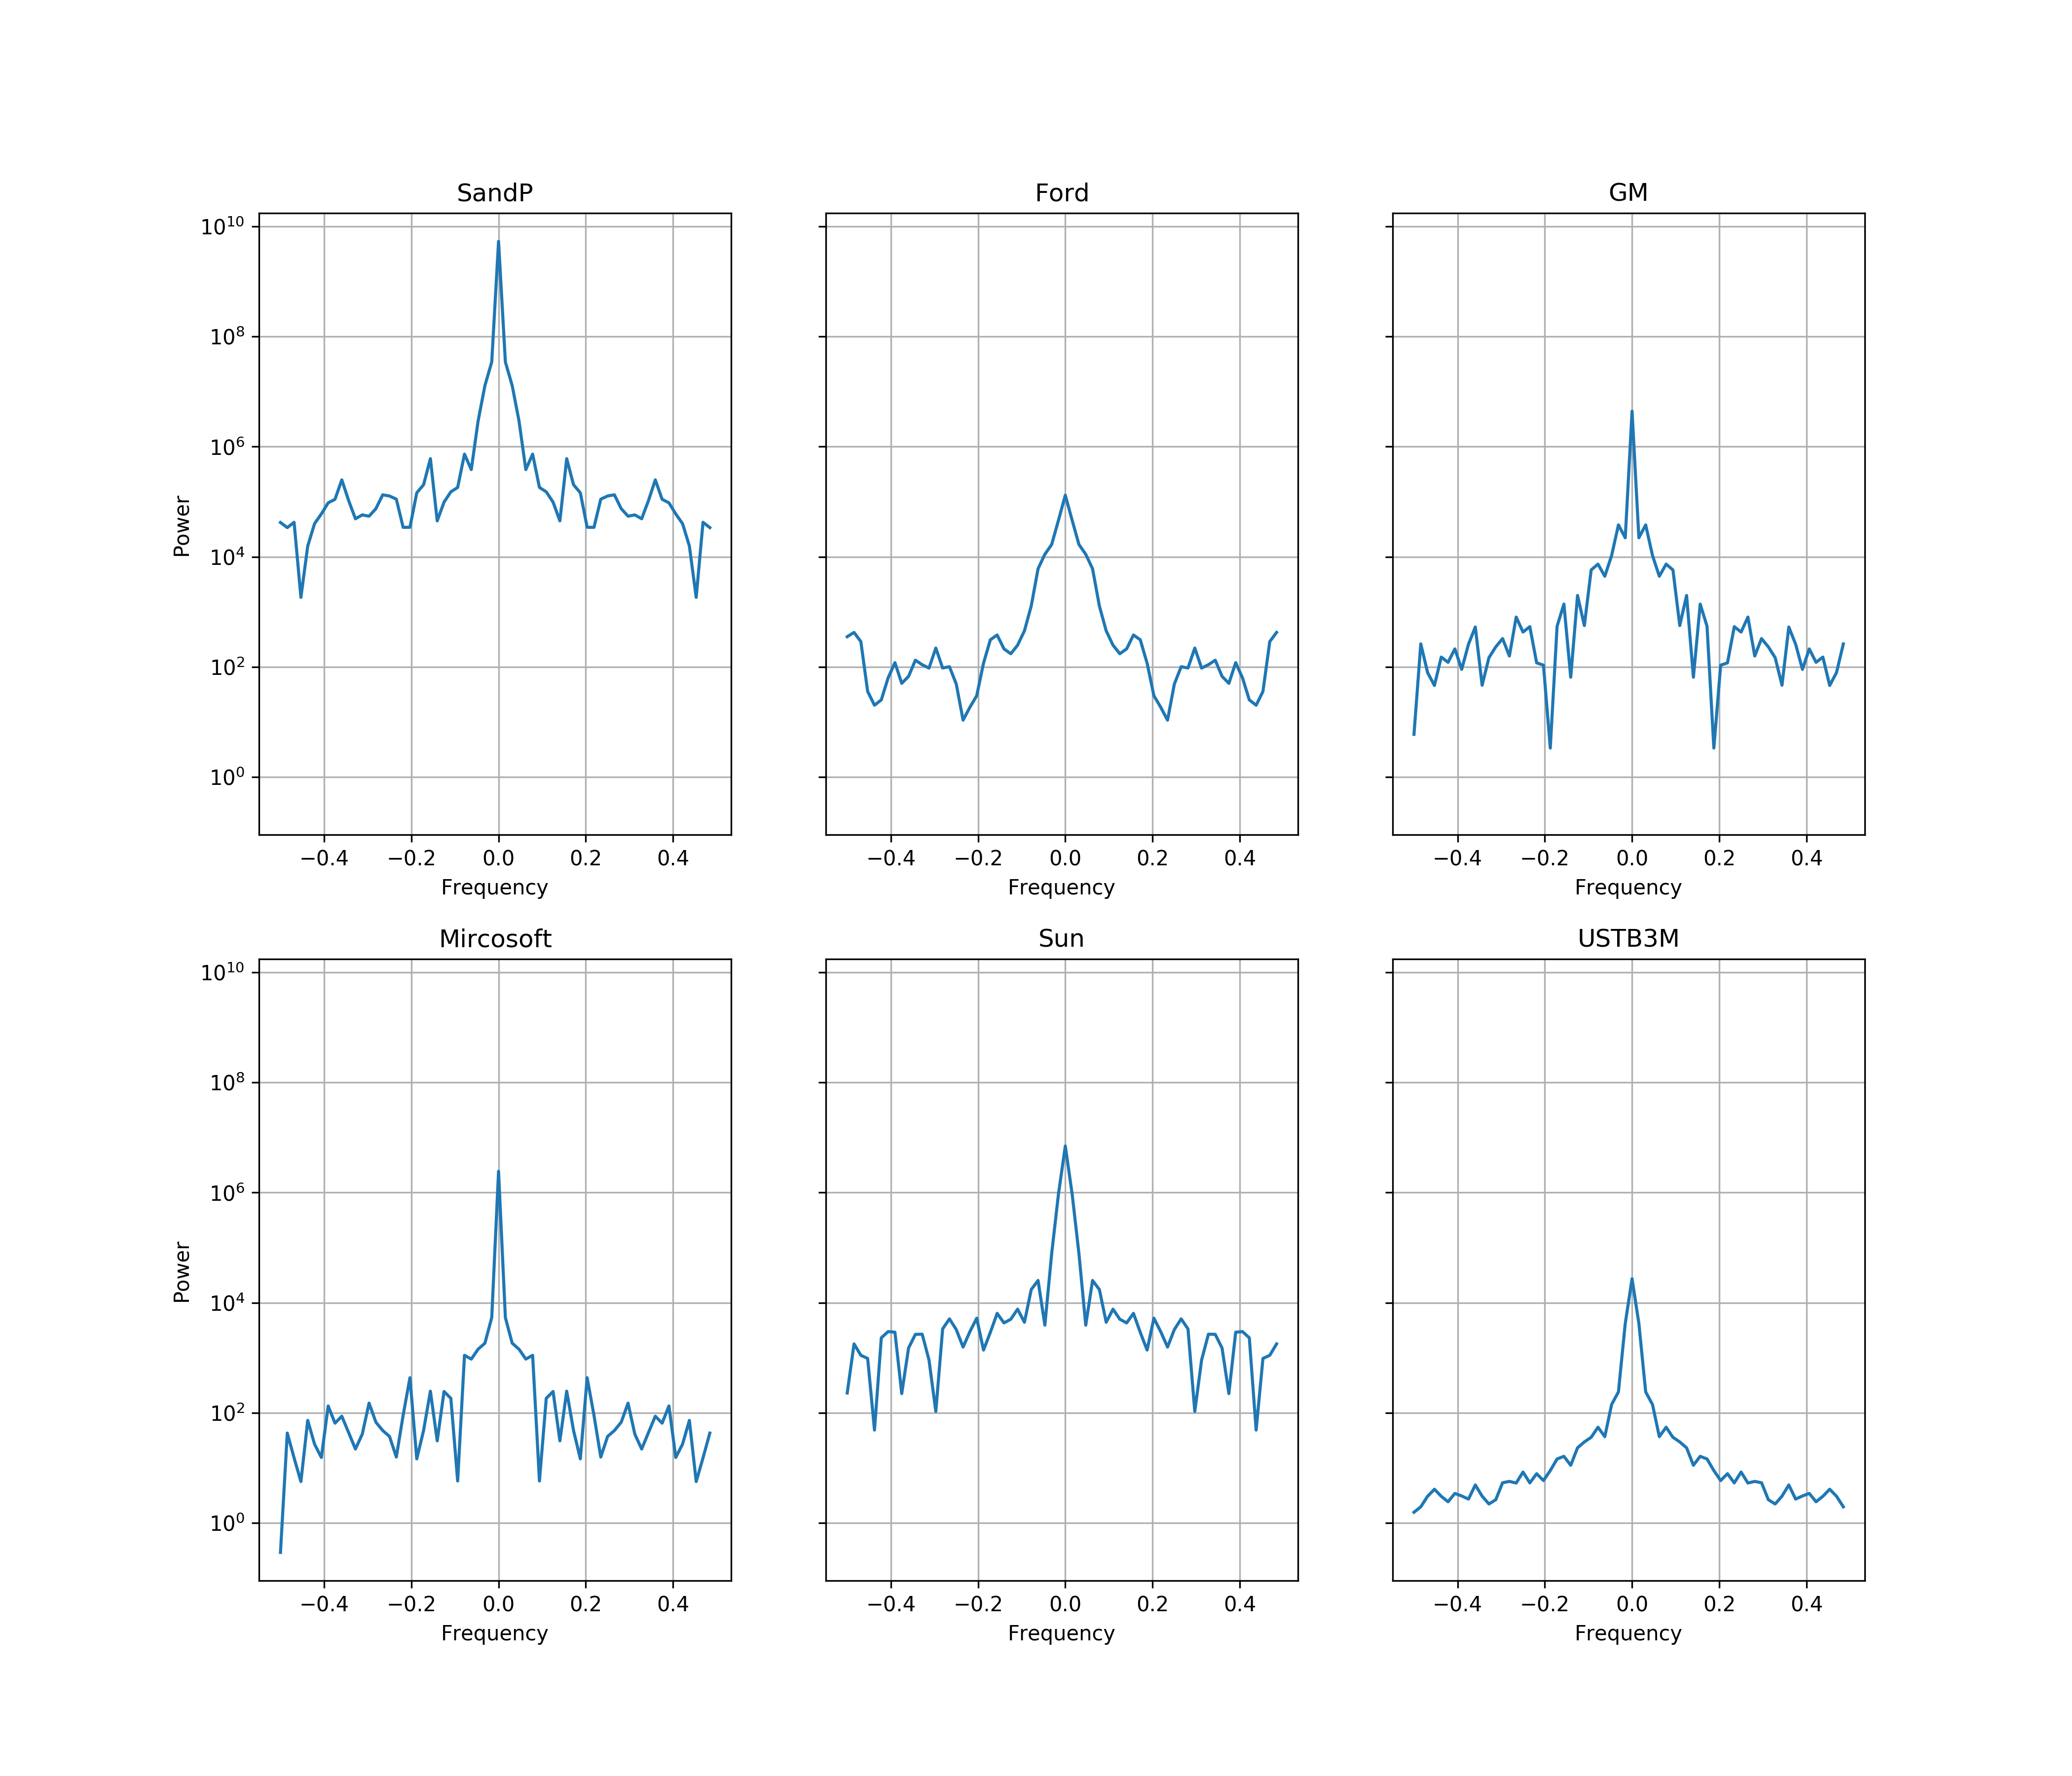
\includegraphics[width=\linewidth]{stocks_power_spectrum.png}
  \caption{
    The power spectra of the compounded returns of six companies. The
    frequencies are in units of per month.
  }
  \label{fig:stocks_ps}
\end{figure*}

Next, we take a look at the daily closing value of the Dow Jones
Industrial Average, which is a measure of the average stock price in
the US market. In figure \ref{fig:dow}, the original data and its
power spectrum are shown. The autocorrelation of the data (figure
\ref{fig:dow_ac} gives some insight onto the direction the market is
headed and when the best time to buy stocks are. At around $200$ days,
the autocorrelation value is approximately zero, meaning that the
market is currently volatile an random. However, as it decreases, the
market follows suit, showing a market crash beginning at around $450$
days as the stock prices continue to fall rapidly. The autocorrelation
begins to ascend when the stock prices are at they're lowest,
indicating that it is the best time to invest in stocks as they begin
rising again.

The power spectrum, on the other hand, seems to indicate
that the dominant frequencies are very small, though there are still
non-negligible contributions from higher frequencies. This suggests
that the market tends to follow larger trends, and that it is best
make long-term investments as they will have the largest potential
growth while short term investments are more likely to go through the
smaller and unpredictable cycles.

\begin{figure*}[t]
  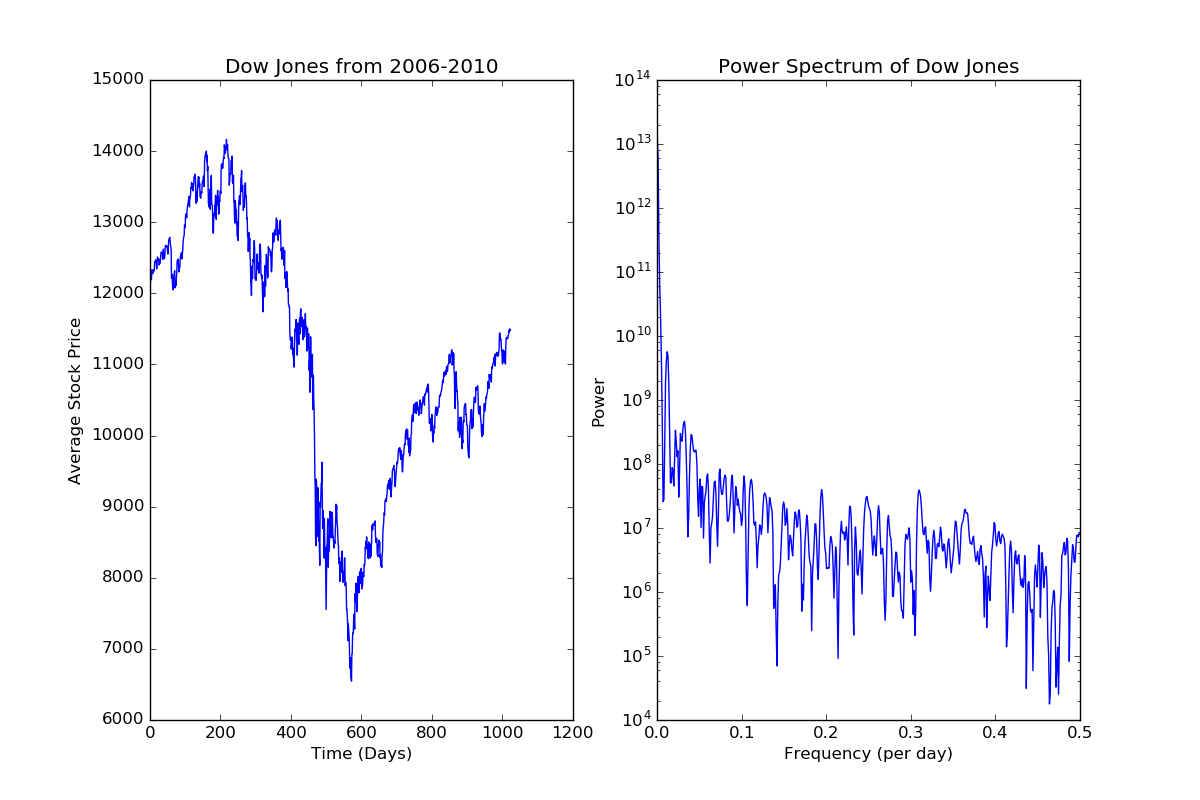
\includegraphics[width=\linewidth]{dow.png}
  \caption{
    The given data of daily average stock prices from $2006$ to $2010$
    is plotted on the left and its power spectrum is given on the
    right. The power spectrum was computed with a Blackman-Harris
    window to minimize leakage.
  }
  \label{fig:dow}
\end{figure*}

\begin{figure}
  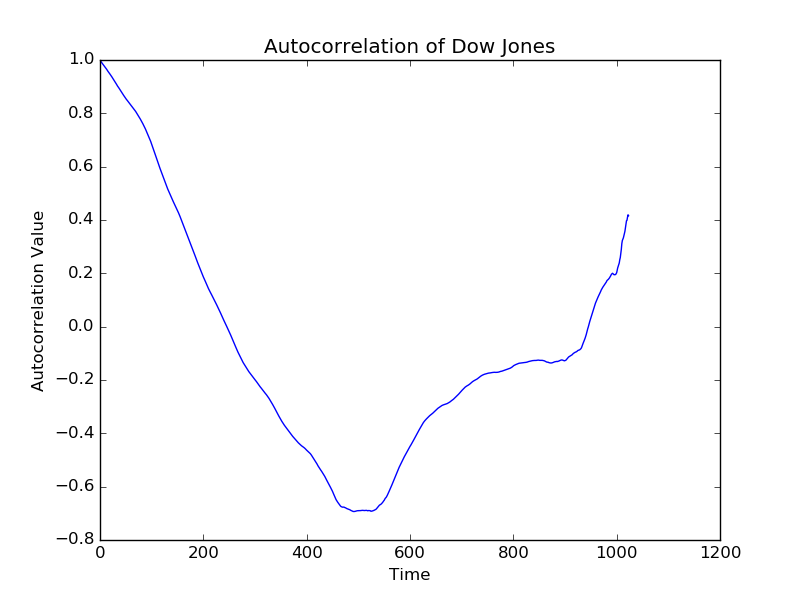
\includegraphics[width=\linewidth]{dow_ac.png}
  \caption{
    The autocorrelation values of the data shown in figure \ref{fig:dow}.
  }
  \label{fig:dow_ac}
\end{figure}

\subsection{Global Warming}
The carbon dioxide is a major component of the air, and may be created and mediated both by natural and anthropogenic processes. Fourier analysis may be used to differentiate between the impacts of natural and anthropogenic processes. A data file of monthly carbon dioxide concentrations was provided for a single location. Some month's data points were not valid concentrations: these points were removed. Monthly data covering 50 years from 1958 to 2008 were used and re-numbered as 'months since March 1958.' Figure \ref{fig:co2trend} shows the data in question. The figure displayed an increase in time, which would prevent fourier analysis of the data. The data were fit to a linear trend, also shown in figure \ref{fig:co2trend}, which was subtracted from the original data to obtain a zero-mean dataset. 

\begin{figure*}
\centering
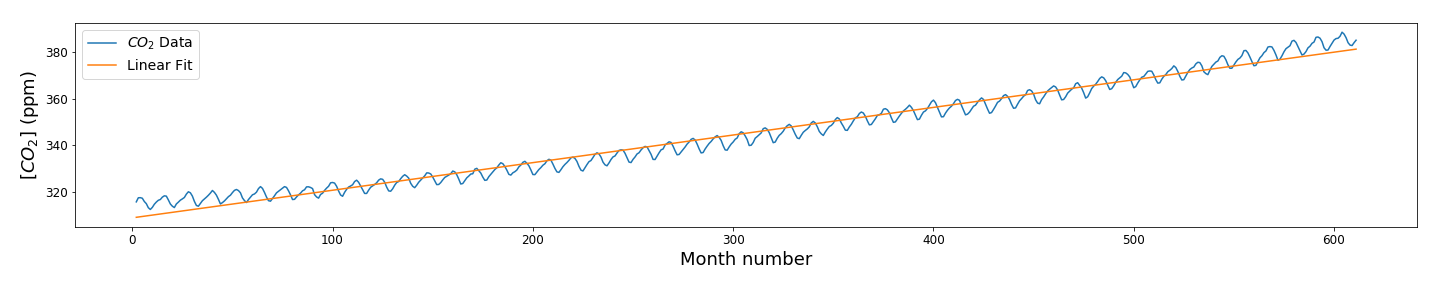
\includegraphics[width=\textwidth]{co2trend}
\caption{Monthly $CO_2$ concentration since March 1958. A linear trendline has been fit to the data using the equation $[CO_2] = 308.8 + 0.118*month$. The line of fit was derived using a least-squares algorithm.}
\label{fig:co2trend}
\end{figure*}

Using the new data set, a power series could be created to analyse periodicity in the data. Since some of the months in the supplied data were missing proper $CO_2$ levels, these points were excluded. Since this made the sampling of the data uneven, a Lomb-Scargle algorithm was used to determine the power spectrum of the data. Figure \ref{fig:co2power} shows the power spectrum. There were two regions of peaks in the spectrum. The first was around the origin. This was likely an artifact of the original data trend. Since the trend was not exactly linear, the linear subtraction did not remove all non-periodic influence. The other peak was located at $f=0.0804 months^{-1}$ or $T=11.90 months$. This was to be expected, as carbon levels should vary seasonally with available plant mass. Where human activity is usually less seasonally correlated, the linear trend in the data was likely anthropogenic.

\begin{figure}
\centering
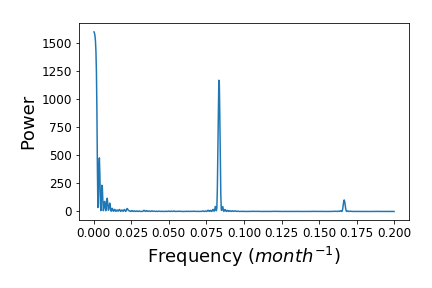
\includegraphics[width=\linewidth]{co2power}
\caption{Power spectrum of $CO_2$ emissions with a linear trend removed.}
\label{fig:co2power}
\end{figure}

Anthropogenic carbon modifies atmospheric properties. Since animal life requires a certain concentration of oxygen in the atmosphere, increasing the carbon dioxide concentration makes the atmosphere increasingly toxic to animals. Assuming that a $10\%$ $[CO_2]$ leads to toxicity, the linear trend indicates that the Earth's atmosphere would become toxic in $841,000$ months or $70,166$ years. This is assuming that all carbon emissions increase at the same rate in the future. This is likely an overestimate in time, since the underlying data was not quite linear. As figure \ref{fig:co2trend} shows, the data appears to be accellerating in its increase relative to a linear trend. This was tested by fitting the data to a quadratic function. If the squared term in the fit was positive this would indicate a positive acceleration. While the quadratic term was very small ($82.8 \times 10^{-6}$), the result was nonetheless positive. 

\section{Discussion}
The DFT is the cornerstone of digital Fourier analysis. It allows a series of data points to be transformed into an equal number of points in Fourier space. By changing the equation into a matrix transformation, the act of transformation becomes much more intuitive. This assignment indirectly demonstrated many properties of the transformation that allow fast Fourier algorithms to be built. First, it was noted that the transformation matrix was symmetric, meaning that it may be computationally solved without computing every element of the matrix, and then apply symmetry. It was also noted that the transformation matrix was the same for any given N. For multiple data sets with the same number of samples, the matrix needs to only be computed once. 

When using a DFT instead of a continuous transform, the rate at which a function is sampled can affect the accuracy of the data in the Fourier space. This is due to the Nyquist frequency, the minimum frequency at which a data set must be sampled to identify all underlying frequencies. This was demonstrated in this assignment by showing that a clearly periodic function appeared to be a constant value to undersampling. This would result in a very different frequency space distribution of a delta function at zero instead of correctly identifying two different underlying frequencies.

When using the DFT, it is often the case that a continuous phenomenon is made discrete by sampling. This can be modeled as using a window that observes a slice of data at a slice in time. The above examples showed that using a standard 'rectangular' window can be problematic, and cause spectral leakage to adjacent frequencies. Two different windows were considered: the Hanning and the Blackman-Harris window. Both windows offered characteristics that were ideal for trying to approximate a narrow peak without tails. The Hanning produced a narrower peak, but the Blackman-Harris produced a better distinction between the peaks and the tails. The choice of window function might depend on application, for instance using a Hanning if one wants a better identification of a single peak, or using a Blackman-Harris if one wants to better distinguish peaks by the small minima created.

Fourier analysis is central to many areas of astrophysics, including orbit identification and stellar activity. In one example a binary system of a pulsar with another star was considered. Light intensity from the stars' location was provided. Given that a binary system is likely to include variable brightness due to one star blocking the other, and that one star was expected to have variable intensity, it was important to be able to separate different periodic properties of the data. When the data were Fourier transformed, there were many strong peaks on the order of seconds with different intensities. There were also some significantly smaller peaks noted throughout the spectrum, including some near $f=0$, corresponding to very long periods. Pulsars can vary significantly in period based on age \cite{pulsar}, making the exact identification of the puslar in the data difficult without further information. However, this example demonstrated that it was fundamental to isolate candidates for either orbiting or pulsar sources. What the problem does demonstrate is the simplicity with which periodicy may be observed.

The human body is based on many different rhythms. The above heart-rate problem showed that this behaviour extends to heart-rate. A heart-rate was found beyond that of the rest rate typical for most people. This suggested that the data may be of a patient with some condition, or in a non-rest state. This shows an important application of heart-rate monitors in the medical field, and how a Fourier analysis tool may be used in the medical field. It was also found that there were frequencies above this present in the data. These frequencies occurred at regular intervals, apparently at integer multiples of the expected frequency. Where the human heart may be heard by listening to the chest, one can recognize that the heart causes vibrations in much the same way as an instrument. Extending this analogy, the further peaks may be an example of harmonics occurring with the heart's vibration. 

Solar activity was another astrophysics application of Fourier analysis. For this example, the data set required padding in order to solve. Thankfully, this padding was already taken care of by modern Fourier transformation libraries in numpy. In actuality, far less padding might have been required than the $954$ padded cell difference between the sample size and $2^{12}$. Instead, many modern algorithms use a combination of powers of 2 and powers of 4 to further optimize the method. The solar data found a period of 130.875 months. This was largely in agreement with the literature \cite{sunspots}. Notably, the highest peak was not the only peak present. A number of other significantly smaller peaks were present, suggesting that there may be other cycles present in sunspots beside the major 11 year cycle. Notably, there was a broad swath of moderate power frequencies around $f=0$. This suggests that there may be some substantially longer solar cycles present. Indeed, Hathaway \cite{sunspots} notes past events of low sub-spot counts centuries ago that were substantially different than modern patterns. Fourier pattern recognition performed better than simply guessing by eye and provided information on patterns that are so long-term they might go unnoticed in time-space.

Climate change has become one of the more important scientific topics of the last decade. Acting as some strange Schroedinger debate, it has managed to simultaneously be a debated and not-debated in the public and academic worlds respectively. It is therefore important to be able to demonstrate the phenomenon as clearly as possible. Figure \ref{fig:co2trend} shows quite clearly an increasing $CO_2$ concentration. Fourier analysis allows further classification of what is happening. Since the data are a combination of both a trend and a periodic pattern, the trend needs to be removed to recover the periodic behaviour. Purely periodic behaviour would be expected, as seasonally changing plant mass provides a natural carbon sink. When a linear trend was applied to the data, the expected periodicity was recovered, along with a slightly broad spread near $f=0$. This indicated that the trend was not entirely removed. This suggests a possible method to model the planet's warming trend. If a trend was proposed that when subtracted completely removed the central peak, it might be a good candidate. A more direct method might involve using the convolution theorem to determine what function in frequency space when convolved with a $f=1/1yr$ function would result in figure \ref{fig:co2power}.

\section{Conclusion}
This assignment successfully demonstrated aspects both of the DFT and FFT, as well as their application to data sets. While the data sets selected were for the most part well-behaved, they illustrated the imperfect nature of data outside of the usually tidy theoretical problems presented in labs. The financial data in particular demonstrated the chaotic nature of real data. This was illustrative: if the real world systems were as clean and intuitive as the examples presented in most texts, there would be no need for the nuanced expertise that the tools we have studied provide. Where unit 1 in this course was focused on finding randomness, this unit was focused on overcoming randomness.


\begin{thebibliography}{00}
	\bibitem{ouyed}
	Ouyed and Dobler, PHYS 581 course notes, Department of Physics and Astrophysics, University of Calgary (2016).
	\bibitem{NR}
	W. Press et al., \emph{Numerical Recipes} (Cambridge University Press, 2010) 2nd. Ed.
	\bibitem{pulsar}
	T. O'Brian, "Properties of Pulsars", University of Manchester Jordell Bank Observatory, accessed at \url{http://www.jb.man.ac.uk/distance/frontiers/pulsars/section1.html}.
	\bibitem{sunspots}
	D. Hathaway, "The Sunspot Cycle",  NASA, accessed at \url{ https://solarscience.msfc.nasa.gov/SunspotCycle.shtml}
\end{thebibliography}

\section{Appendix}
For access to the source codes used in this project, please visit \url{https://github.com/Tsintsuntsini/PHYS_581} for a list of files and times of most recent update.
	
\end{document}